\documentclass{article}
\usepackage{graphicx} % Required for inserting images

\usepackage{amsmath}
\usepackage{bm}
\usepackage{soul}
\usepackage{siunitx}

\usepackage{booktabs}

\title{Rocket Linear Dynamics}
\author{alessandro.zavoli }
\date{October 2023}

\newcommand{\vinf}{v_\infty}


 

\begin{document}



\maketitle

% \begin{abstract}
%     TBD
% \end{abstract}

\section{Introduction}

Tisserand plot can help understand the effects and potential gain of one (or multiple) flybys.

This analysis assumes that the secondary body (pedix ``s'') flies in a circular orbit about the primary body (pedix ``p'')

Also, we denotes distance from the primary body with upper-case  $R$, wherease distances in the Sphere of Influence (SOI) of the secondary body with lower-case $r$.



We consider only the ($R_P$, $R_P$) Tisserand plot.



First, we show that we can cover the plot by iso-$v_\infty$ contour lines.


In fact, each pair ($R_P$, $R_A$) corresponds to a unique pair ($\vinf$, $\alpha$)



Let $V_{sc}$ be the spacecraft velocity and $V$


\begin{align}
    V_{sc}^2 = V_s^2 + \vinf^2 + 2 V_s \vinf \cos\alpha
\end{align}
with $V_s = \sqrt{\mu_p/r_s}$

\begin{align}
    a = (R_P + R_A)/2 \\
    e = 1- rp/a \\
    \cos\nu = (p-r_s)/(e r_s) \\
%
    V_{sc,r} = \sqrt{\frac{\mu_p}{p}} e \sin\nu \\
    V_{sc,t} = \sqrt{\frac{\mu_p}{p}} (1+e\cos\nu) \\
    V_{sc} = \sqrt{V_{sc,r}^2+V_{sc,t}^2}
    \\
    v_{\infty,r} = V_r \\
    v_{\infty,t} = V_t - V_s \\
    \vinf = \sqrt{v_{\infty,r}^2+v_{\infty,t}^2} \\
    \alpha = \arccos\frac{V_{sc}^2-V_s^2-\vinf^2}{2V_{sc}\vinf}
\end{align}

The inverse transform follows the same reasoning

\begin{align}
    V_{sc}^2 &= V_s^2 + \vinf^2 + 2 V_s \vinf \cos\alpha\\
     % v_{\infty,r} = \vinf \sin\alpha\\
     % v_{\infty,t} = \vinf \cos\alpha\\
     % V_{sc,r} = v_{\infty,r} \\
     % V_{sc,t} = V_s + v_{\infty,t}\\
     V_{sc,r} &= \vinf \sin\alpha\\
     V_{sc,t} &= V_s + \vinf \cos\alpha\\
     a &= \dfrac{\mu_p/2}{\dfrac{V_{sc}^2}{2}-\dfrac{\mu_p}{R_s}}\\
     h &= R_s V_{sc,t} \\
     e &= \sqrt{1-\frac{h^2}{\mu a}}\\
     R_P &= a(1-e)\\
    R_A &= a(1+e)
\end{align}



Using the inverse transform it is possible to draw lines (iso-contours) of constant $\vinf$,
fixing $\vinf=\bar{v}_\infty$ and
varying $\alpha \in [0, \pi]$.

Iso-contours of $alpha$ can also be plotted as dashed lines. These lines are obtained fixing the values of $\alpha$ (e.g., $\alpha=0$, 15°, 30°, ..., 180°). and varying $\vinf \in [0, v_{\infty_\text{max}}]$.


\hl{FIGURA 1}
 

As an alternative, one can draw lines of constant period (of the spacecraft orbit around the primary body), for a given $n:m$ resonance.
These iso-contours appears a straight lines in the ($R_A$, $R_P$). 
In fact, $R_P+R_A = 2 a$, wuth $a$ constant if the period is constat, being $a = ^3\sqrt{\left(\frac{T}{2\pi}\right)^2\mu_p}$.

For a resontant orbit, one hase $T_{sc}:T_s = n:m$, hence
\begin{align}
    a_{sc} = a_s (\frac{n}{m})^{2/3}
\end{align}
Thus, the iso-resonant lines are found for a specific choice of $n:m$ calculating the pairs ($R_A$, $R_P$) varying the eccentricity from 0 to 1 (or $e_\text{max}$.
\begin{align}
    R_P = a_s (\frac{n}{m})^{2/3} \left(1-e\right)\\
    R_A = a_s (\frac{n}{m})^{2/3} \left(1+e\right)
\end{align}

\newpage
\begin{figure}[!htbp]
    \centering
    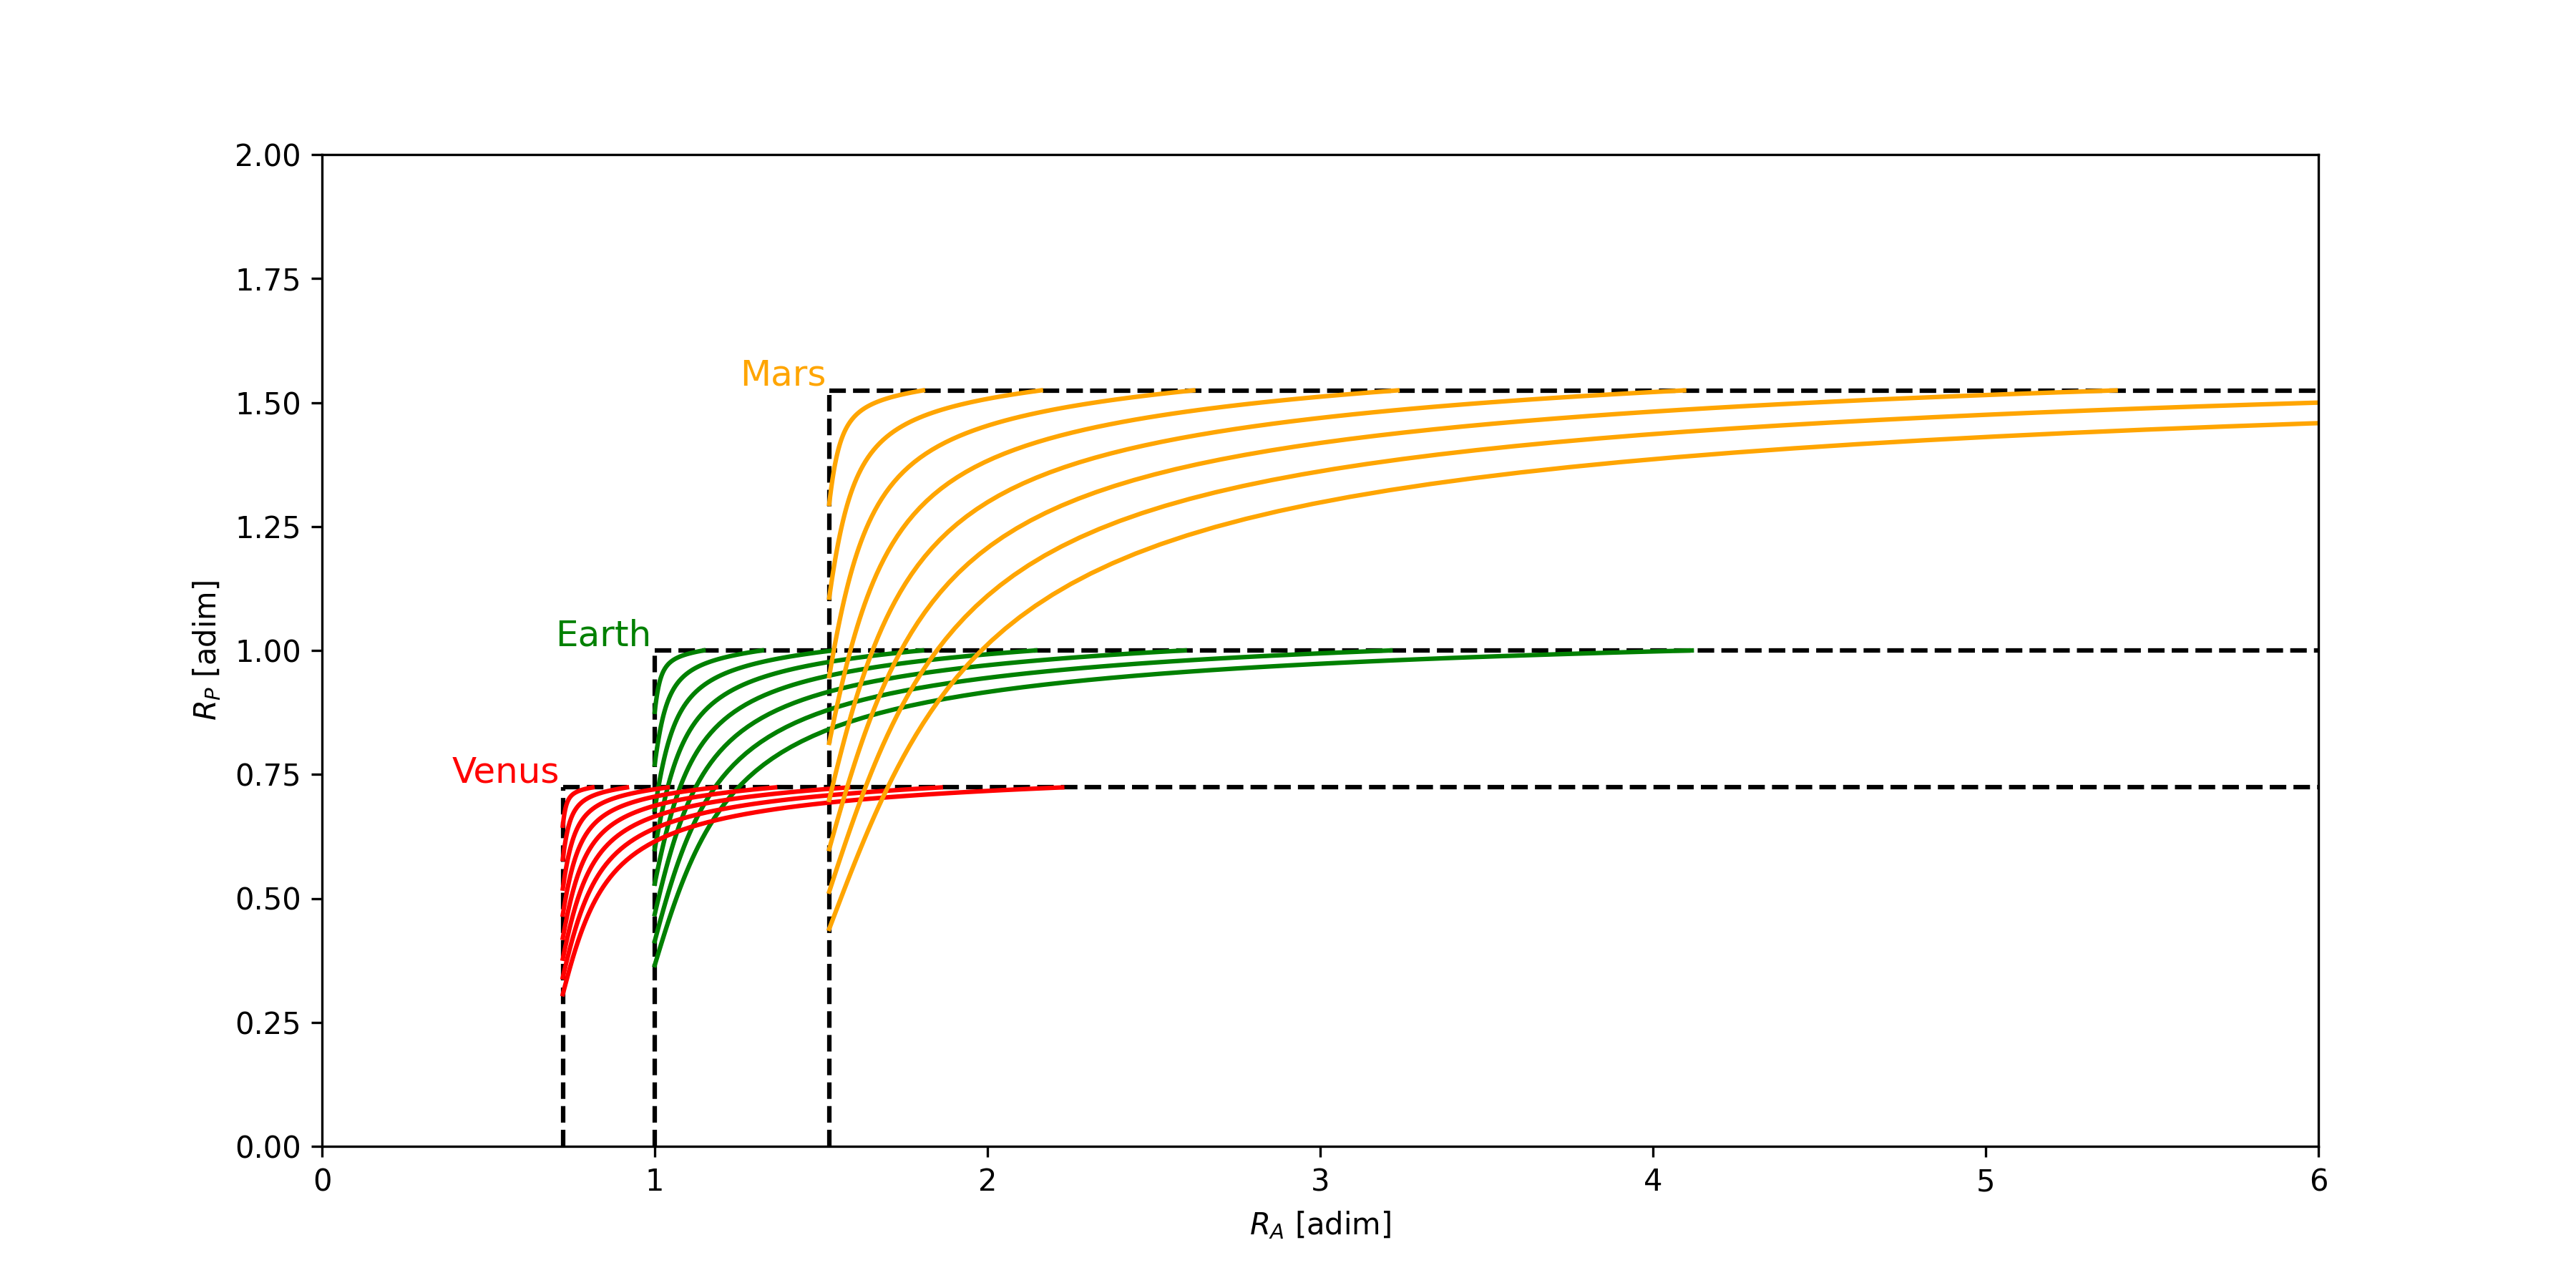
\includegraphics[width=\linewidth]{Figures/tisserand_solar.png}
    \caption{Tisserand plot for the Solar system.}
    \label{fig:tisserand_solar}
\end{figure}

\begin{figure}[!htbp]
    \centering
    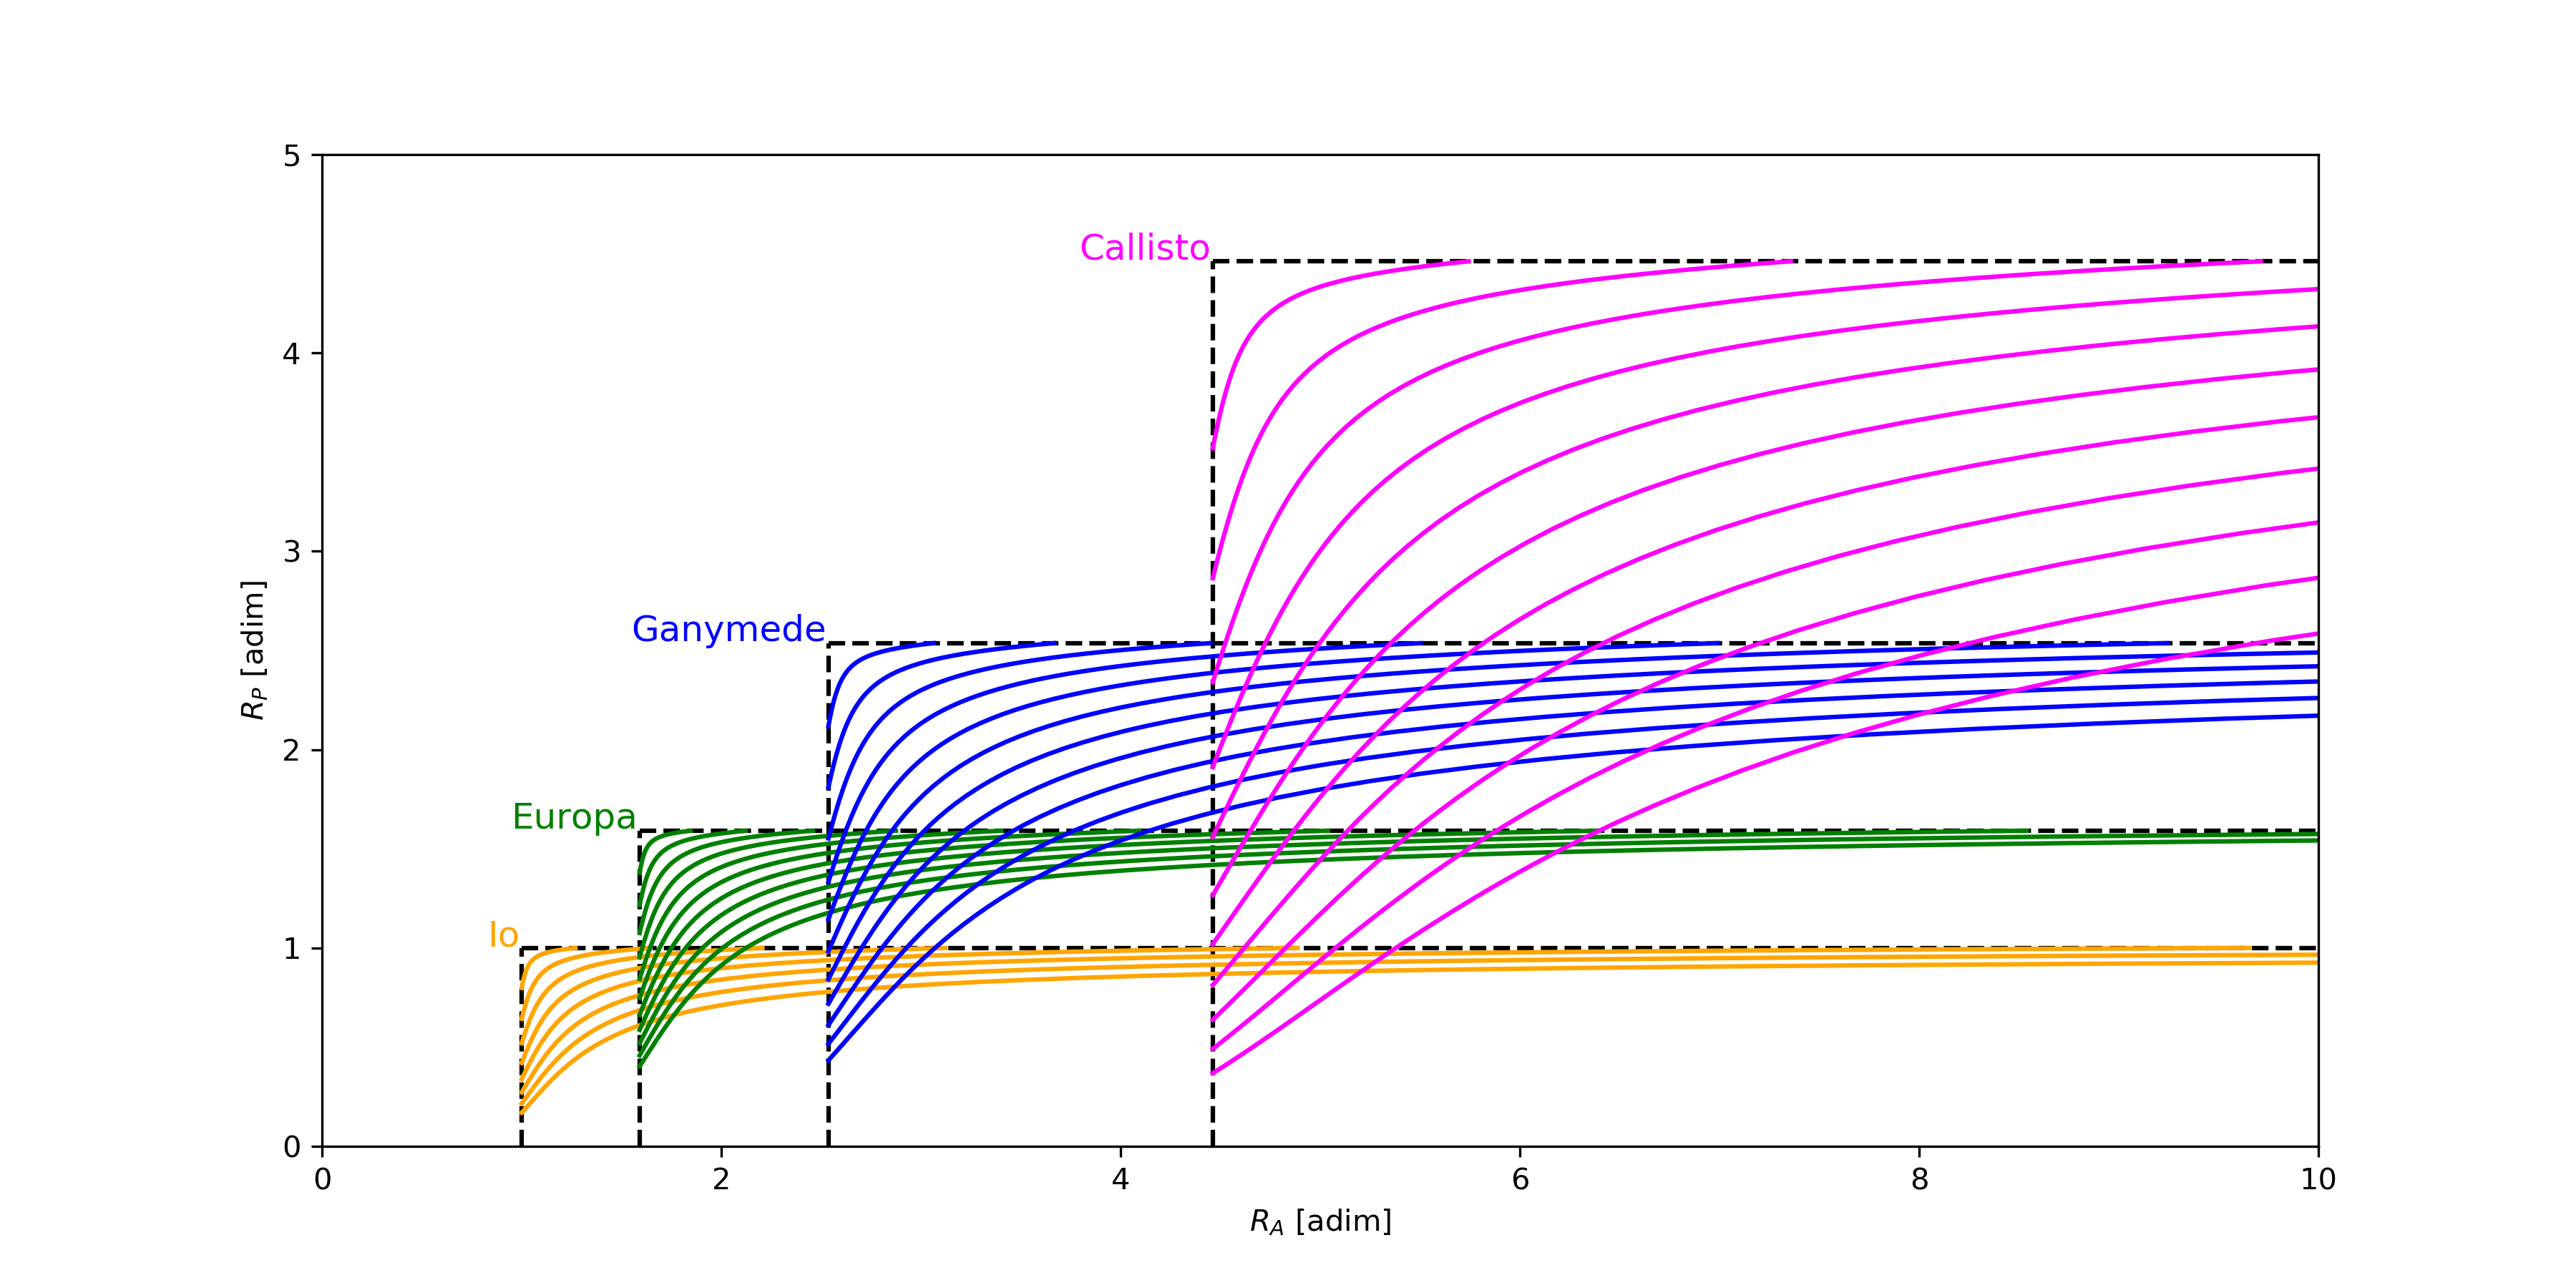
\includegraphics[width=\linewidth]{Figures/tisserand_jovian.png}
    \caption{Tisserand plot for the Jovian system.}
    \label{fig:tisserand_jovian}
\end{figure}






\begin{figure}[!htbp]
    \centering
    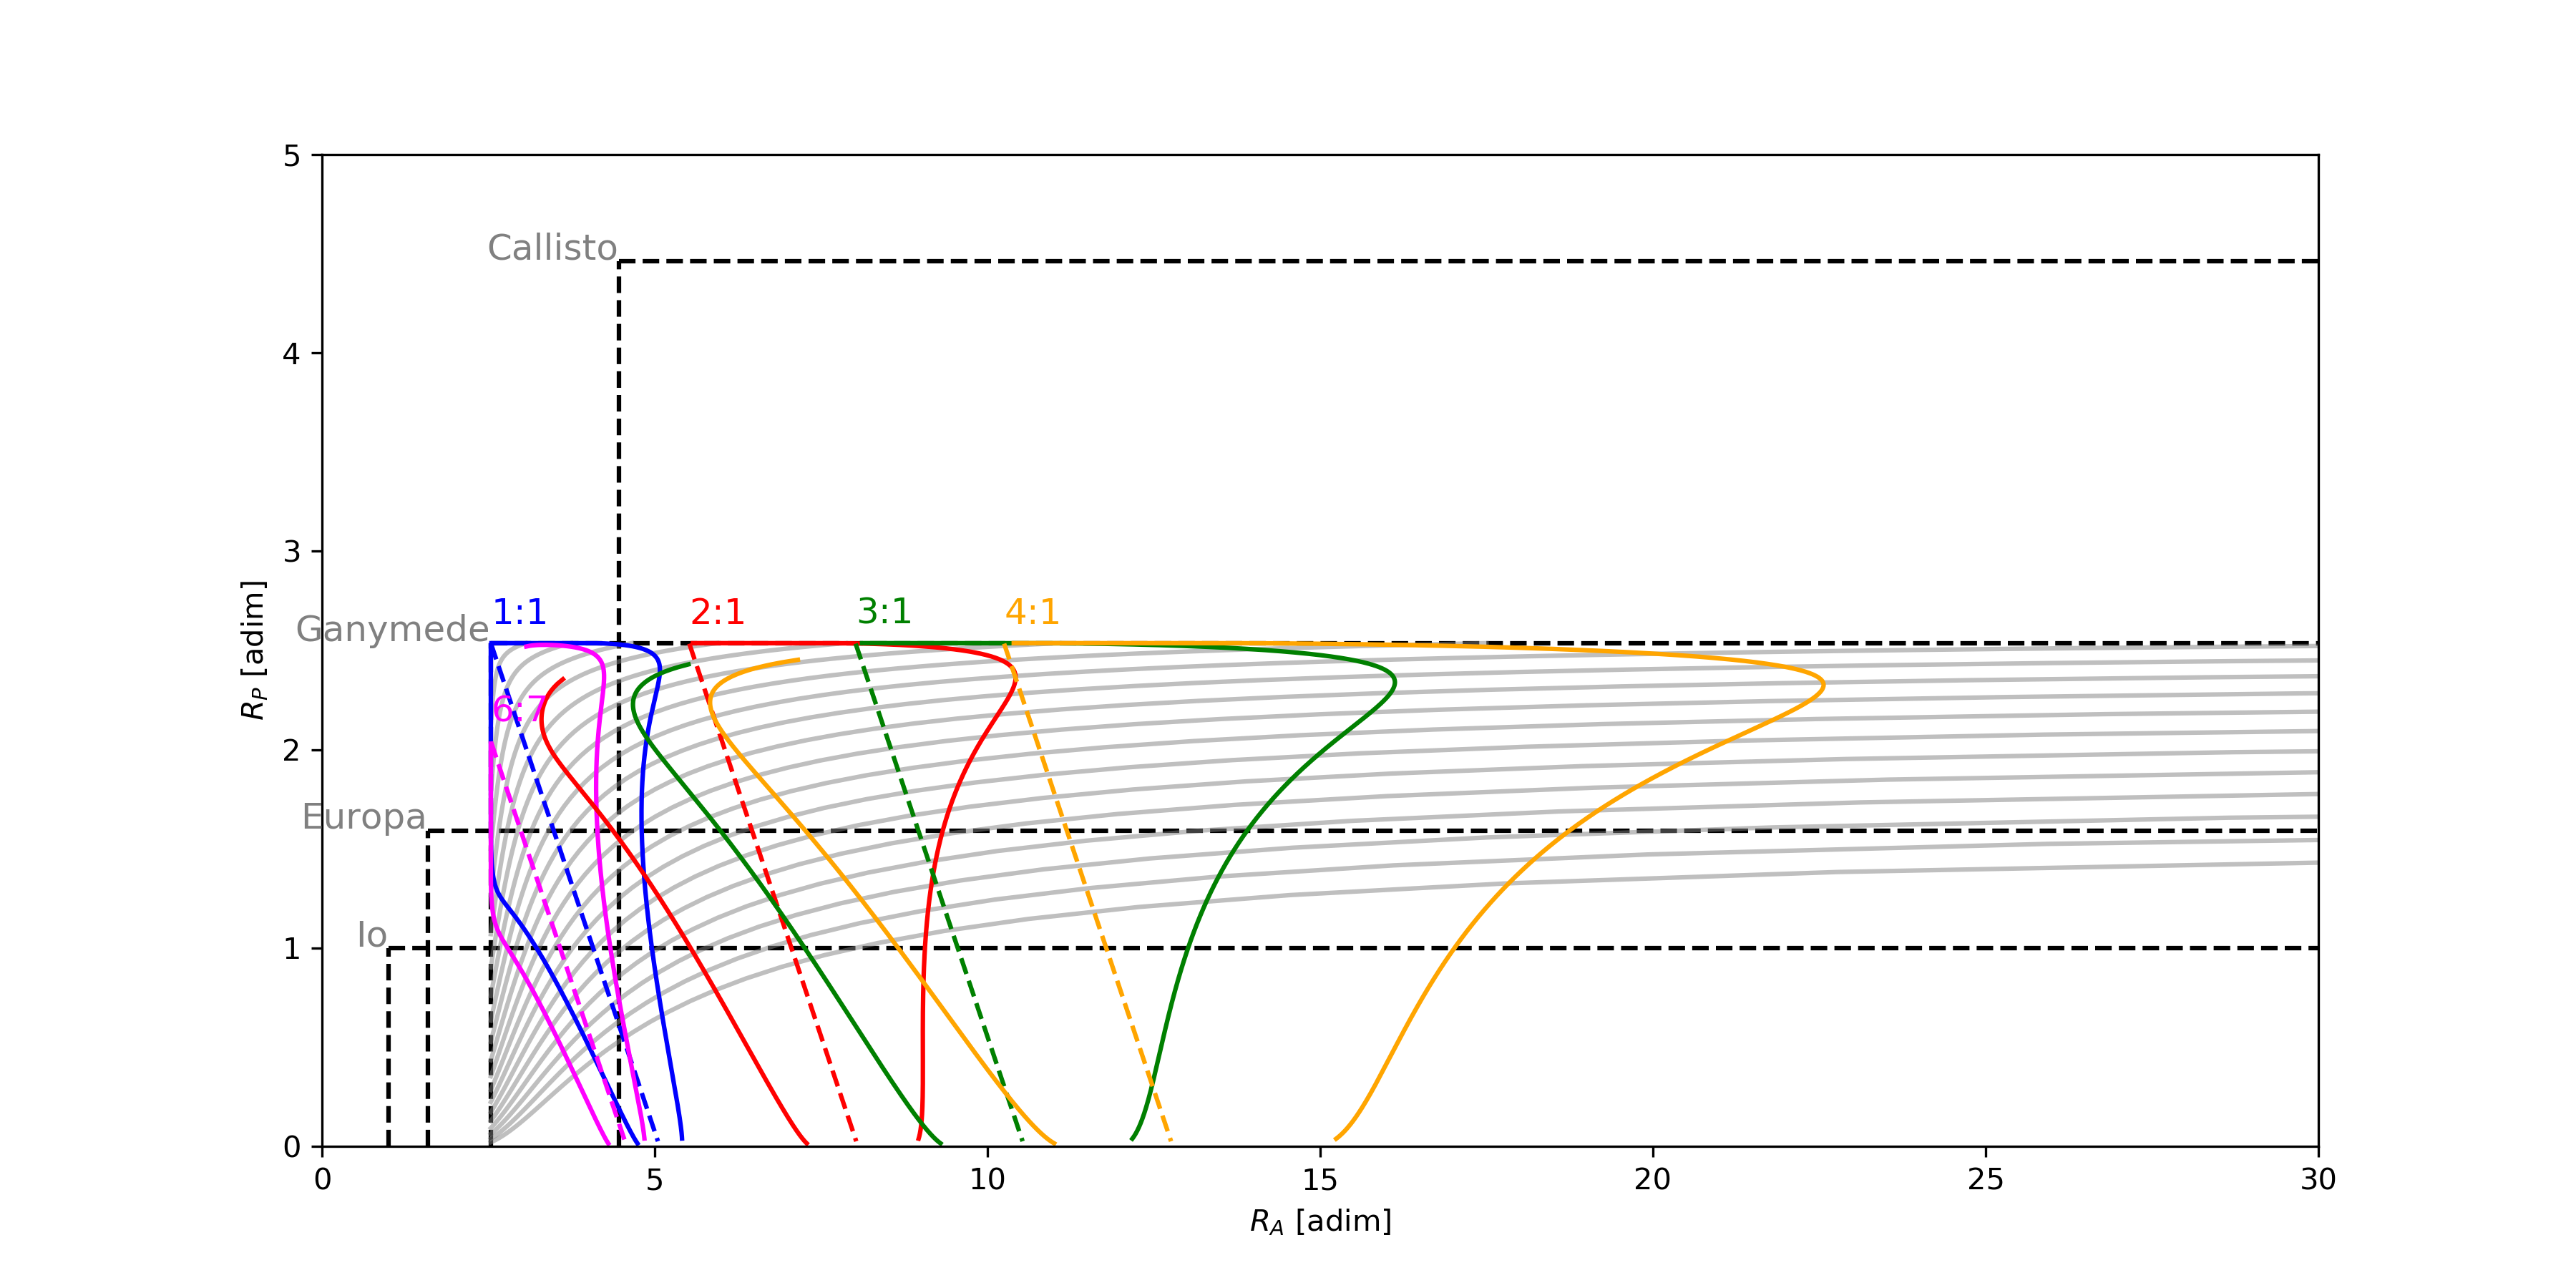
\includegraphics[width=\linewidth]{Figures/tisserand_jovian_resonance.png}
    \caption{Tisserand plot for the Solar system.}
    \label{fig:tisserand_jovian_resonance}
\end{figure}




The effect of a flyby corrsponds to an instantaneous change of velocity.
This means a jump on the Tisserand plot.
Note that the $\vinf$ is not altered by a flyby, thus the points before and after the flyby must be located on the same iso-$\vinf$ contour line.

The amount of displacement along the  $\vinf$ contour line depends on the change of the pump angle between the conditions after ($\alpha_+$) and before ($\alpha_-$) the flyby.
Their difference is equal to the deflection angle $\delta$

\begin{equation}
    \bm{v}_{\infty-}^T \cdot \\bm{v}_{\infty+} = \vinf^2 \cos\delta
\end{equation}

\hl{figura del triangolo di velocita'}

The deflection angle $\delta$, can be found as

\begin{equation}
    \sin\frac{\delta}{2} = \frac{\mu_s/r_{flyby}}{\vinf^2+\mu_s/r_{flyby}}
\end{equation}

where $r_{flyby}$ is the pericenter radius of the planetocentric hyperbola, that is, the flyby radius.










\end{document}
